%%%%%%%%%%%%%%%%%%%%%%%%%%%%%%%%%%%%%%%%%
% Beamer Presentation
% LaTeX Template
% Version 1.0 (10/11/12)
%
% This template has been downloaded from:
% http://www.LaTeXTemplates.com
%
% License:
% CC BY-NC-SA 3.0 (http://creativecommons.org/licenses/by-nc-sa/3.0/)
%
%%%%%%%%%%%%%%%%%%%%%%%%%%%%%%%%%%%%%%%%%

%----------------------------------------------------------------------------------------
%	PACKAGES AND THEMES
%----------------------------------------------------------------------------------------

\documentclass{beamer}

\mode<presentation> {

% The Beamer class comes with a number of default slide themes
% which change the colors and layouts of slides. Below this is a list
% of all the themes, uncomment each in turn to see what they look like.

%\usetheme{default}
%\usetheme{AnnArbor}
%\usetheme{Antibes}
%\usetheme{Bergen}
%\usetheme{Berkeley}
%\usetheme{Berlin}
%\usetheme{Boadilla}
%\usetheme{CambridgeUS}
%\usetheme{Copenhagen}
%\usetheme{Darmstadt}
%\usetheme{Dresden}
%\usetheme{Frankfurt}
%\usetheme{Goettingen}
%\usetheme{Hannover}
%\usetheme{Ilmenau}
%\usetheme{JuanLesPins}
%\usetheme{Luebeck}
\usetheme{Madrid}
%\usetheme{Malmoe}
%\usetheme{Marburg}
%\usetheme{Montpellier}
%\usetheme{PaloAlto}
%\usetheme{Pittsburgh}
%\usetheme{Rochester}
%\usetheme{Singapore}
%\usetheme{Szeged}
%\usetheme{Warsaw}

% As well as themes, the Beamer class has a number of color themes
% for any slide theme. Uncomment each of these in turn to see how it
% changes the colors of your current slide theme.

%\usecolortheme{albatross}
%\usecolortheme{beaver}
%\usecolortheme{beetle}
%\usecolortheme{crane}
%\usecolortheme{dolphin}
%\usecolortheme{dove}
%\usecolortheme{fly}
%\usecolortheme{lily}
%\usecolortheme{orchid}
%\usecolortheme{rose}
%\usecolortheme{seagull}
%\usecolortheme{seahorse}
%\usecolortheme{whale}
%\usecolortheme{wolverine}

%\setbeamertemplate{footline} % To remove the footer line in all slides uncomment this line
%\setbeamertemplate{footline}[page number] % To replace the footer line in all slides with a simple slide count uncomment this line

%\setbeamertemplate{navigation symbols}{} % To remove the navigation symbols from the bottom of all slides uncomment this line
}

\usepackage{graphicx} % Allows including images
\usepackage{booktabs} % Allows the use of \toprule, \midrule and \bottomrule in tables

%----------------------------------------------------------------------------------------
%	TITLE PAGE
%----------------------------------------------------------------------------------------

\title[ARQUS 2021]{Talk on ARQUS : Cyber-Security Summmer School 2021} % The short title appears at the bottom of every slide, the full title is only on the title page
\titlegraphic{
    
\includegraphics[width=3cm]{images/UJM-logo.png}
    \hspace{2cm}
    
\includegraphics[width=3cm]{images/Arqus-EU-tris.png}
}
\author{Kushagra Singh BISEN} % Your name
\institute[Universit\'e de Lyon] % Your institution as it will appear on the bottom of every slide, may be shorthand to save space
{
Universit\'e de Lyon          \\ % Your institution for the title page
\medskip
\textit{kushagra.bisen@etu.univ-st-etienne.fr} % Your email address
}
\date{\today} % Date, can be changed to a custom date

\begin{document}

\begin{frame}
\titlepage % Print the title page as the first slide
\end{frame}

\begin{frame}
\frametitle{Overview} % Table of contents slide, comment this block out to remove it
\tableofcontents % Throughout your presentation, if you choose to use \section{} and \subsection{} commands, these will automatically be printed on this slide as an overview of your presentation
\end{frame}

%----------------------------------------------------------------------------------------
%	PRESENTATION SLIDES
%----------------------------------------------------------------------------------------

%------------------------------------------------
\section{Introduction}

\begin{frame}
    \frametitle{Introduction}
    I am Kushagra Singh BISEN, a MSc student in Cyber-Physical Social Systems student at 
    Universit\'e de Lyon. I present you my work during the days 6-9 September in the Cyber-Security Summmer
    School organized by Arqus European University Alliance \cite{p1}.  \newline
    During the course of 4 days, we were taught different aspects to cyber-security from researchers of different partner universites 
    and were given quizzes and challenges to assess our understanding of the concepts.
\end{frame}

\section{Challenges}
\subsection{Security and Privacy in Android}
\begin{frame}
    \frametitle{Security and Privacy in Android}
    Security and Privacy is analyzed using two different softwares,
    \begin{itemize}
        \item RiskInDroid
        \item SPECK
    \end{itemize}
The application to be analyzed was 'xiaomi home app'. Xiaomi home apps are famous for asking for too many permissions, evenif they don't need those.
An example of such could be, the home light application asking permissions to access the contacts, and camera. Such extra permissions can be used to spy/sell the data
for data mining purposes. This makes us to use softwares to analyze the \textbf{APK} file before 
installing it to our system.
\end{frame}

\begin{frame}
    \frametitle{RiskInDroid}
    Dockerfile is used to run the analysis application. The apk file is selected to result in a score out of 100
    based upon different classifiers. The resulting score value is \textbf{30.34 / 100}.
    Regarding the permissions, 
    \begin{itemize}
        \item Declared Permissions - 58
        \item Required and Used Permissions - 21
        \item Required and not Used Permissions - 37
        \item Not required but used permissions - 4
    \end{itemize}

    Developers can analyze each and every permission, and make decisions or modify the apk for our use.
\end{frame}

\begin{frame}
    \frametitle{RiskInDroid}
    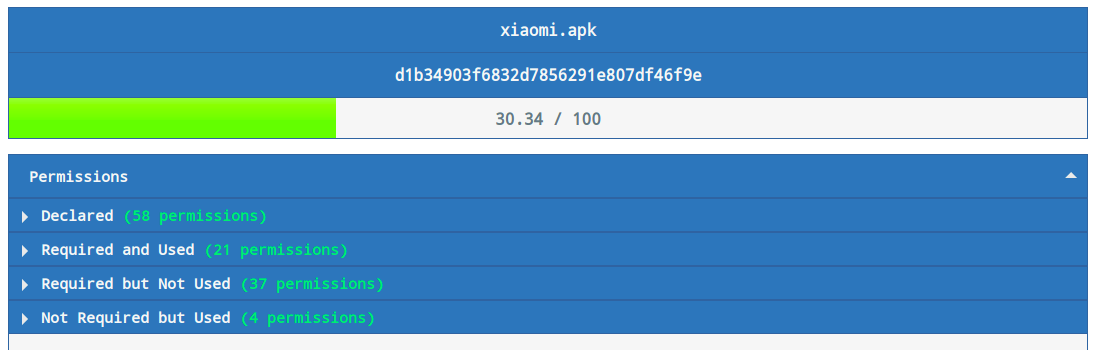
\includegraphics[width=\textwidth]{images/xiaomi-riskinDroid.png}
\end{frame}

\begin{frame}
    \frametitle{SPECK}
    The application is downloaded from Github and built using gradle. The python script analyzes the code written in the application, to display the quality of code written with respect to 
    the security of the application. 1719 files were analyzed and code was displayed in 3 classifiers, \textit{INFO, WARNING and CRITICAL}. There are 32 rules which are employed
    for the analysis, and when you execute they analyze files which depend on the rule. An example of the rule can be, "Store private data within internal storage". Manifest files and main java file are given 
    % recommendations to change the application's features to improve the security. An example of the recommendation is, "* Don't use SharedPreferences objects to share data
    % - at line 244  'return context.getSharedPreferences("multidex.version", Build.VERSION.SDK_INT < 11 ? 0 : 4);"
\end{frame}

\subsection{Cyber-Security Challenges}
\begin{frame}
    \frametitle{Cyber-Security Challenge}
    The challenge consists the exploitation of a buffer overflow. Unfortunately, I was not able to solve the challenge. 
\end{frame}

\subsection{Introduction to UNIX \& Quizzes}
\begin{frame}
    \frametitle{UNIX Quizzes}
    There were various quizzes given related to file management, networking, file editors, I/O management. 
    I solved the quizzes from section 1 to section 7.
    Unfortunately, I could not solve the 'init.d' quiz completely, I did solve only 3 of those questions.
    I could not find the catalog files in my workstation.
\end{frame}

\subsection{Side Channel Analyis with Deep Learning}
\begin{frame}
    \frametitle{Side Channel Analyis with Deep Learning}
In this section, I was able to understand and learn Simple Power Analyis. I could not understand Differential Power Analyis and further modules to an extent where I could solve questions related to them.
\end{frame}
\section{Conclusion}
\subsection{What I learnt?}
\begin{frame}
    \frametitle{What I learnt?}
At the end of the summer school, I discovered that Cyber Security is much more than hacking a webpage or getting access to a server. Including Physics, Quantum computing to solve cyber Security
problems as well as employing deep learning for cyber-security was a great insight. I wish to rewatch the recordings which will be shared after the school to better understand the concepts
to employ later.
\end{frame}
\begin{frame}
    \frametitle{References}
    \footnotesize{
    \begin{thebibliography}{99}

    % "Home: Arqus." Arqus European Alliance. Accessed September 09, 2021. https://www.arqus-alliance.eu/

    \bibitem[Home : Arqus]{p1} ARQUS (2021)
    \newblock \emph{Arqus European Alliance}. Accessed September 09, 2021. https://www.arqus-alliance.eu/
    
%    \bibitem[B. R. Barricelli, E. Casiraghi and D. Fogli, 2019]{p2} Barricelli et al. (2019)
%    \newblock A Survey on Digital Twin: Definitions, Characteristics, Applications, and Design Implications
%    \newblock \emph{IEEE Access}, vol. 7, pp. 167653-167671, 2019, doi: 10.1109/ACCESS.2019.2953499

%     \bibitem[Koenig, N. and Howard, A.]{p3} Koenig et al. (2004)
%     \newblock Design and use paradigms for Gazebo, an open-source multi-robot simulator
%     \newblock \emph{2004 IEEE/RSJ International Conference on Intelligent Robots and Systems (IROS) (IEEE Cat. No.04CH37566)}

    \end{thebibliography}
    }
\end{frame}



\begin{frame}
{\centerline{Thank you for your attention. Any questions?}}
\begin{center}

\includegraphics[width=0.6\textwidth]{images/questions.png}
\end{center}
\end{frame}

%----------------------------------------------------------------------------------------

\end{document} 